\chapter{Perceptron and the multilayer perceptron}
\label{ch:perceptron}

Every network in this book, from a two-layer classifier to a Transformer with a
hundred layers, is built from one object: a weighted sum followed by a fixed
non-linear function. This chapter takes that object apart, shows exactly what one
of them can and cannot do (the XOR story that OAs keep asking about), and then
stacks them into the multilayer perceptron whose parameters we learn to count
in our sleep.

\section{The artificial neuron}
\prototype{Inputs $\x=(0.5,-1,2)$, weights $\w=(0.4,0.3,-0.2)$, bias $b=0.1$:
the neuron outputs $\phi(\w\T\x+b)$ for some transfer function $\phi$.}

\subsection{Definition}
\begin{definition}
	An \vocab{artificial neuron} with weights $\w\in\RR^d$, bias $b\in\RR$ and
	\vocab{activation} (or \vocab{transfer}) function $\phi:\RR\to\RR$ maps an
	input $\x\in\RR^d$ to
	\[ a = \phi(z), \qquad z = \w\T\x + b = \textstyle\sum_{i=1}^d w_i x_i + b. \]
	The number $z$ is the \vocab{pre-activation} (or weighted sum, or logit);
	$a$ is the \vocab{activation}.
\end{definition}

The classical choices of $\phi$ are the \vocab{step} (Heaviside) function
$\ind{z\ge 0}$, the \vocab{sigmoid} $\sigma(z)=1/(1+e^{-z})$, $\tanh z$ and the
\vocab{ReLU} $\max(0,z)$. \Cref{ch:activations} compares them properly; for now
they are just four ways to squash or clip $z$.

\begin{center}
\begin{tikzpicture}[x=1cm,y=1cm]
	\foreach \i/\lab in {1/x_1,2/x_2,3/x_3} {
		\node[inneuron] (x\i) at (0,2-\i) {$\lab$};
	}
	\node[inneuron, fill=gray!15] (one) at (0,-2) {$1$};
	\node[op, minimum size=9mm, circle] (sum) at (3,0) {$\Sigma$};
	\node[op, minimum width=12mm] (phi) at (5,0) {$\phi(\cdot)$};
	\node (a) at (6.8,0) {$a$};
	\draw[flow] (x1) -- node[above, sloped, font=\footnotesize] {$w_1$} (sum);
	\draw[flow] (x2) -- node[above, sloped, font=\footnotesize] {$w_2$} (sum);
	\draw[flow] (x3) -- node[above, sloped, font=\footnotesize] {$w_3$} (sum);
	\draw[flow] (one) -- node[below, sloped, font=\footnotesize] {$b$} (sum);
	\draw[flow] (sum) -- node[above, font=\footnotesize] {$z$} (phi);
	\draw[flow] (phi) -- (a);
\end{tikzpicture}
\end{center}

\begin{example}[One neuron, four transfer functions]
	\label{ex:neuron}
	With the prototype numbers, $z = 0.4(0.5)+0.3(-1)+(-0.2)(2)+0.1 =
	\gv{c01_perceptron/neuron_z}$. Then
	\begin{center}
		\begin{tabular}{lcccc}
			\toprule
			$\phi$ & step & sigmoid & $\tanh$ & ReLU \\
			\midrule
			$a=\phi(z)$ & $\gv{c01_perceptron/neuron_step}$ & $\gv{c01_perceptron/neuron_sigmoid}$ &
			$\gv{c01_perceptron/neuron_tanh}$ & $\gv{c01_perceptron/neuron_relu}$ \\
			\bottomrule
		\end{tabular}
	\end{center}
	All four agree with \pt{torch.sigmoid}, \pt{torch.tanh} and \pt{torch.relu}
	(checked in \script{c01_perceptron}). OA version: inputs
	$(1,0,1,1)$, weights $(0.6,-0.9,-0.4,0.5)$, bias $-0.3$, sigmoid transfer. Then
	$z=\gv{c01_perceptron/q_z}$ and the output is $\sigma(z)=\gv{c01_perceptron/q_sig}$.
	The input that is $0$ contributes nothing whatever its weight, which is
	exactly what the setter hopes you will forget.
\end{example}

\begin{remark}
	\trap The neuron applies $\phi$ to the weighted sum; it does not take a
	weighted sum of $\phi(x_i)$. A second common slip is dropping the bias: then
	every decision boundary is forced through the origin.
\end{remark}

\subsection{The biological analogy, and where it breaks}
The name comes from a cartoon of a cortical neuron: dendrites collect signals
from other cells, synapses scale them (the weights), the cell body integrates
them (the sum), and the axon fires if the total crosses a threshold (the step
function). The cartoon is useful for exactly one sentence. It breaks almost
everywhere an interviewer might push:
\begin{itemize}
	\ii Real neurons communicate with spikes in time; information sits in rates
	and timing, not in one real number per forward pass.
	\ii Dendrites themselves compute non-linear functions, so one biological
	neuron is closer to a small network than to one unit.
	\ii Nobody has shown that the brain runs backpropagation: it would need the
	backward pass to reuse the forward weights exactly (``weight transport'').
	\ii An artificial neuron with a sigmoid is literally logistic regression
	(see the logistic-regression chapter of the companion book
	\otherbook{Classical Machine Learning}); the interesting behaviour comes from
	composing many of them and training them jointly.
\end{itemize}
\begin{moral}
	A neuron is a linear function followed by a fixed scalar non-linearity.
	Everything else is composition.
\end{moral}

\section{The perceptron}
\prototype{Six labelled points in the plane; Rosenblatt's rule adds misclassified
points to $\w$ until every point is on the right side.}

\subsection{The algorithm}
Rosenblatt's perceptron \cite{rosenblatt} is a step-function neuron
$\hat y = \sign(\w\T\x+b)$ with labels $y\in\{-1,+1\}$ and a learning rule that
only reacts to mistakes.

\begin{algo}[Perceptron]
	Initialise $\w=\zero$, $b=0$. Repeat over the data until an epoch makes no
	mistake: if $y_i(\w\T\x_i+b)\le 0$ then
	$\w \gets \w + \eta\, y_i \x_i$ and $b\gets b+\eta\, y_i$.
\end{algo}

Why it is the right direction: after the update the new margin of the same point
is $y_i(\w+\eta y_i\x_i)\T\x_i + y_i(b+\eta y_i) = y_i(\w\T\x_i+b)+\eta(\norm{\x_i}^2+1)$,
strictly larger than before. The rule is stochastic (sub)gradient descent on the
\vocab{perceptron loss} $\ell(\w,b)=\max\bigl(0,-y(\w\T\x+b)\bigr)$, whose
gradient is $-y\x$ on a mistake and $0$ otherwise.

\codefile[code/dl/c01\_perceptron.py]{gen/dl/snip/c01_perceptron-perceptron.py}

\begin{example}[A full trace]
	\label{ex:perceptron-trace}
	Data: \gv{c01_perceptron/data_list}; $\eta=1$, points visited in index order.
	Every update made:
	\begin{center}
		\begin{tabular}{cccc}
			\toprule
			epoch & mistake on & $\w$ after & $b$ after \\
			\midrule
			\gv{c01_perceptron/trace_rows}
			\bottomrule
		\end{tabular}
	\end{center}
	Epoch $\gv{c01_perceptron/n_epochs}$ makes no mistake, so the algorithm stops
	after $\gv{c01_perceptron/n_updates}$ updates at
	$\w=(\gv{c01_perceptron/w1},\gv{c01_perceptron/w2})$,
	$b=\gv{c01_perceptron/bfin}$. The result is identical to
	\pt{sklearn.linear\_model.Perceptron(eta0=1, shuffle=False)}, which the script
	asserts. Notice $\x_2$ and $\x_5$, the two points closest to each other with
	opposite labels, cause every update after the first.
\end{example}

\begin{center}
\begin{tikzpicture}
\begin{axis}[napkinplot, width=0.6\linewidth, height=0.5\linewidth,
	xlabel=$x_1$, ylabel=$x_2$, xmin=-3.5, xmax=3.5, ymin=-3.5, ymax=3.5,
	axis lines=middle, legend pos=outer north east]
	\addplot[only marks, mark=*, blue!80!black] table[x=x1,y=x2] {gen/dl/data/c01_perceptron-pos.dat};
	\addlegendentry{$y=+1$}
	\addplot[only marks, mark=square*, red!80!black] table[x=x1,y=x2] {gen/dl/data/c01_perceptron-neg.dat};
	\addlegendentry{$y=-1$}
	\addplot[black, thick] table[x=x,y=y] {gen/dl/data/c01_perceptron-line.dat};
	\addlegendentry{final $\w\T\x+b=0$}
\end{axis}
\end{tikzpicture}
\end{center}

\begin{remark}
	\trap ``Increase the learning rate to make the perceptron converge faster.''
	With $\w_0=\zero$, every weight vector the algorithm visits is $\eta$ times the
	one it visits with $\eta=1$, so the signs of all predictions, the mistakes and
	the number of updates are identical. The script reruns the trace with $\eta=0.1$
	and asserts the final weights are exactly $0.1$ times the ones above. The
	learning rate of the perceptron only matters when $\w_0\neq\zero$.
\end{remark}

\subsection{The convergence theorem}
\begin{theorem}[Perceptron convergence]
	Suppose $\norm{(\x_i,1)}\le R$ for all $i$ and some unit vector $\w^\star$
	(acting on augmented inputs $(\x,1)$) satisfies $y_i\,{\w^\star}\T(\x_i,1)\ge\gamma>0$ for all
	$i$. Then the perceptron makes at most $(R/\gamma)^2$ updates, whatever the
	order of the data.
\end{theorem}
\begin{proof}
	Absorb $b$ into $\w$ by appending $1$ to every input, and take $\eta=1$ (by the
	remark above this costs nothing). Let $\w_k$ be the weights after $k$ updates,
	the $k$-th made on example $i$. Two inequalities:
	\begin{itemize}
		\ii Progress: $\w_k\T\w^\star = \w_{k-1}\T\w^\star + y_i\x_i\T\w^\star
		\ge \w_{k-1}\T\w^\star + \gamma$, so $\w_k\T\w^\star\ge k\gamma$.
		\ii Bounded growth: $\norm{\w_k}^2 = \norm{\w_{k-1}}^2 + 2y_i\w_{k-1}\T\x_i +
		\norm{\x_i}^2 \le \norm{\w_{k-1}}^2 + R^2$ because the update happened only
		when $y_i\w_{k-1}\T\x_i\le 0$. So $\norm{\w_k}^2\le kR^2$.
	\end{itemize}
	By Cauchy--Schwarz $k\gamma\le\w_k\T\w^\star\le\norm{\w_k}\le\sqrt{k}R$, hence
	$k\le(R/\gamma)^2$.
\end{proof}

\begin{example}[How loose is the bound?]
	For the six points above, $R=\gv{c01_perceptron/R}$ and the best possible
	margin (from a hard-margin linear SVM, normalised) is
	$\gamma=\gv{c01_perceptron/gamma}$, so the bound is
	$(R/\gamma)^2\approx\gv{c01_perceptron/bound}$ updates. The perceptron needed
	$\gv{c01_perceptron/n_updates}$. The bound is a worst case over orderings and is
	driven by the single tightest pair of points.
\end{example}

\begin{ques}
	Why does the rule update when $y_i(\w\T\x_i+b)\le 0$ rather than $<0$? (Start
	from $\w=\zero$.)
\end{ques}

\begin{remark}
	\trap The theorem says nothing about non-separable data, where the perceptron
	never stops, and nothing about \emph{which} separator it returns: unlike an
	SVM it does not maximise the margin, and the answer depends on the order of
	the data.
\end{remark}

\section{XOR: what one neuron cannot do}
\prototype{$\mathrm{XOR}(x_1,x_2)$ is $1$ exactly when one input is $1$; no
line separates $\{(0,1),(1,0)\}$ from $\{(0,0),(1,1)\}$.}

\begin{proposition}
	No single step-function neuron computes XOR.
\end{proposition}
\begin{proof}
	Suppose $\ind{w_1x_1+w_2x_2+b\ge 0}$ equals XOR. The four inputs give
	$b<0$, $w_1+w_2+b<0$, $w_2+b\ge 0$ and $w_1+b\ge 0$. Adding the last two,
	$w_1+w_2+2b\ge 0$, so $w_1+w_2+b\ge -b>0$, contradicting the second.
\end{proof}

The same argument works for any monotone $\phi$ thresholded at any level, so
``use a sigmoid instead'' does not help: a single neuron's decision boundary is
always a hyperplane. This observation, made precise by Minsky and Papert
\cite{minsky}, is the usual one-line answer to ``why do we need hidden layers?''.

\begin{example}[The perceptron on XOR]
	Running the perceptron for $\gv{c01_perceptron/xor_epochs}$ epochs on XOR
	(labels $\pm1$) gives $\gv{c01_perceptron/xor_total}$ updates in total and never
	fewer than $\gv{c01_perceptron/xor_min_mistakes}$ mistakes in an epoch: the
	weights cycle forever. \pt{sklearn}'s perceptron ends at training accuracy
	$\gv{c01_perceptron/xor_sklearn_acc}$, no better than a coin.
\end{example}

\subsection{Two layers solve it by hand}
XOR $=$ OR and not AND. Each of OR and AND is linearly separable, and so is
``$h_1$ and not $h_2$'' once $h_1,h_2$ are available as features:

\codefile[code/dl/c01\_perceptron.py]{gen/dl/snip/c01_perceptron-xor_hand.py}

\begin{center}
\begin{minipage}{0.47\linewidth}
\centering
\begin{tikzpicture}[x=1.1cm,y=1.1cm]
	\node[inneuron] (x1) at (0,1) {$x_1$};
	\node[inneuron] (x2) at (0,-1) {$x_2$};
	\node[hidneuron] (h1) at (2,1) {$h_1$};
	\node[hidneuron] (h2) at (2,-1) {$h_2$};
	\node[outneuron] (o) at (4,0) {$\hat y$};
	\draw[flow] (x1) -- node[above, font=\scriptsize] {$1$} (h1);
	\draw[flow] (x1) -- node[pos=0.25, above, font=\scriptsize] {$1$} (h2);
	\draw[flow] (x2) -- node[pos=0.25, below, font=\scriptsize] {$1$} (h1);
	\draw[flow] (x2) -- node[below, font=\scriptsize] {$1$} (h2);
	\draw[flow] (h1) -- node[above, font=\scriptsize] {$+1$} (o);
	\draw[flow] (h2) -- node[below, font=\scriptsize] {$-1$} (o);
	\node[font=\scriptsize, above=1mm of h1] {$b=-0.5$};
	\node[font=\scriptsize, below=1mm of h2] {$b=-1.5$};
	\node[font=\scriptsize, above=1mm of o] {$b=-0.5$};
\end{tikzpicture}
\end{minipage}\hfill
\begin{minipage}{0.47\linewidth}
\centering
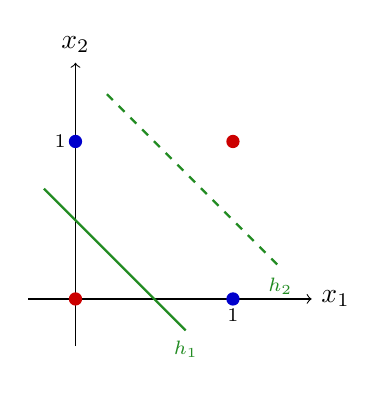
\begin{tikzpicture}[scale=2.0]
	\draw[->] (-0.3,0) -- (1.5,0) node[right] {$x_1$};
	\draw[->] (0,-0.3) -- (0,1.5) node[above] {$x_2$};
	\draw[ForestGreen, thick] (-0.2,0.7) -- (0.7,-0.2) node[below, font=\scriptsize] {$h_1$};
	\draw[ForestGreen, thick, dashed] (0.2,1.3) -- (1.3,0.2) node[below, font=\scriptsize] {$h_2$};
	\fill[red!80!black] (0,0) circle (1.2pt) (1,1) circle (1.2pt);
	\fill[blue!80!black] (0,1) circle (1.2pt) (1,0) circle (1.2pt);
	\node[font=\scriptsize, left] at (0,1) {$1$};
	\node[font=\scriptsize, below] at (1,0) {$1$};
\end{tikzpicture}
\end{minipage}
\end{center}

\begin{center}
	\begin{tabular}{cc|cc|c}
		\toprule
		$x_1$ & $x_2$ & $h_1=\text{OR}$ & $h_2=\text{AND}$ & $\hat y$ \\
		\midrule
		\gv{c01_perceptron/xor_rows}
		\bottomrule
	\end{tabular}
\end{center}
The hidden layer \emph{re-represents} the input: in $(h_1,h_2)$ coordinates the
four points become $(0,0)$, $(1,0)$, $(1,0)$, $(1,1)$ and the two classes are
linearly separable. That is the whole idea of representation learning in one
table.

\begin{example}[Can gradient descent find it?]
	Train a 2-$H$-1 network with $\tanh$ hidden units and a sigmoid output on the
	four XOR points with Adam, from $\gv{c01_perceptron/xor_seeds}$ random
	initialisations. With $H=2$ (the minimum that can represent XOR)
	$\gv{c01_perceptron/xor_solved2}$ of the $\gv{c01_perceptron/xor_seeds}$ runs
	reach $100\%$ accuracy; the rest stall in a poor local configuration. With
	$H=8$, $\gv{c01_perceptron/xor_solved8}$ of $\gv{c01_perceptron/xor_seeds}$
	succeed. Over-parameterising makes the optimisation problem easier, a theme
	that returns with every large model in this book.
\end{example}

\section{The multilayer perceptron}
\prototype{A 784-256-128-10 ReLU network for MNIST digits has
$\gv{c01_perceptron/mlp_params}$ parameters.}

\subsection{Forward pass and shapes}
A \vocab{multilayer perceptron} (MLP, also \vocab{fully connected} or
\vocab{dense} network) with layer widths $n_0,n_1,\dots,n_L$ computes
\[
	\h^{(0)}=\x,\qquad
	\z^{(l)} = \W^{(l)}\h^{(l-1)}+\bb^{(l)},\qquad
	\h^{(l)}=\phi\bigl(\z^{(l)}\bigr)\quad(l=1,\dots,L),
\]
with $\W^{(l)}\in\RR^{n_l\times n_{l-1}}$ and $\bb^{(l)}\in\RR^{n_l}$. The last
layer usually has no $\phi$ (it outputs logits; \cref{ch:activations}). With a batch
$\X\in\RR^{B\times n_0}$ stored row-wise, as every framework does, the same layer
reads $\mathbf{Z}=\X\W\T+\one\bb\T$, shape $\shp{B,n_l}$; PyTorch's
\pt{nn.Linear(n\_in, n\_out)} stores \pt{weight} with shape \shp{n\_out, n\_in} for
exactly this reason.

\begin{proposition}[Parameter count]
	An MLP with widths $n_0,\dots,n_L$ has $\sum_{l=1}^L (n_{l-1}+1)\,n_l$
	parameters: each of the $n_l$ units in layer $l$ has $n_{l-1}$ weights and one
	bias.
\end{proposition}

\begin{example}[Counting an MNIST MLP]
	For $784\to256\to128\to10$:
	$785\cdot256 = \gv{c01_perceptron/mlp_l1}$,
	$257\cdot128 = \gv{c01_perceptron/mlp_l2}$,
	$129\cdot10 = \gv{c01_perceptron/mlp_l3}$; total
	$\gv{c01_perceptron/mlp_params}$, equal to
	\pt{sum(p.numel() for p in model.parameters())} for the PyTorch model. A 3-4-2
	network has $\gv{c01_perceptron/small_params}$ parameters, a typical one-line OA
	item. Activation functions and the input layer have no parameters.
\end{example}

\codefile[code/dl/c01\_perceptron.py]{gen/dl/snip/c01_perceptron-count.py}

\subsection{Why the non-linearity is not optional}
Delete every $\phi$ and the network collapses:
$\W^{(2)}(\W^{(1)}\x+\bb^{(1)})+\bb^{(2)} = (\W^{(2)}\W^{(1)})\x +
(\W^{(2)}\bb^{(1)}+\bb^{(2)})$, a single affine map, however many layers you stack
(the script checks this numerically). A deep linear network can represent only
what one linear layer can, so it cannot solve XOR either.

\begin{remark}
	\trap ``ReLU is linear, so it adds no non-linearity.'' ReLU is \emph{piecewise}
	linear: it is linear on each side of $0$ but not linear overall
	($\relu(-1)+\relu(1)\neq\relu(0)$). A ReLU network is a piecewise-linear function
	with possibly a huge number of pieces, which is exactly what the next section
	exploits.
\end{remark}

\section{Universal approximation, and why depth still matters}
\prototype{Thirty-two ReLU units in one hidden layer approximate
$\sin(2\pi t)+t/2$ on $[0,1]$ to within $\gv{c01_perceptron/uat_err32}$.}

\begin{theorem}[Universal approximation, informal]
	Let $\phi$ be continuous and not a polynomial. For every continuous
	$f:K\to\RR$ on a compact $K\subset\RR^d$ and every $\eps>0$ there is a network
	with one hidden layer of $\phi$ units and a linear output whose output is within
	$\eps$ of $f$ everywhere on $K$.
\end{theorem}
Cybenko proved it for sigmoids \cite{cybenko}; later work extended it to any
continuous non-polynomial activation. Two caveats make up the interview answer:
the theorem says a suitable width \emph{exists} but not how large it is (it can be
exponential in $d$), and it says nothing about whether gradient descent will find
the weights or whether they generalise.

\subsection{A constructive proof in one dimension}
With ReLUs the 1-D case is a construction you can write in an interview. Take
knots $0=t_0<t_1<\dots<t_n=1$ and the piecewise-linear interpolant of $f$. Its slope
on $[t_{k},t_{k+1}]$ is $s_k$. Then
\[
	\hat f(t) = f(0) + \sum_{k=0}^{n-1} a_k\,\relu(t-t_k),\qquad
	a_0=s_0,\ a_k=s_k-s_{k-1},
\]
because the unit $\relu(t-t_k)$ switches on at $t_k$ and changes the slope by
$a_k$ there. That is a one-hidden-layer network with $n$ units: hidden weights $1$,
hidden biases $-t_k$, output weights $a_k$.

\codefile[code/dl/c01\_perceptron.py]{gen/dl/snip/c01_perceptron-relu_interp.py}

\begin{center}
\begin{tikzpicture}
\begin{axis}[napkinplot, width=0.62\linewidth, height=0.42\linewidth,
	xlabel=$t$, legend pos=south west, ymin=-1.2, ymax=1.5]
	\addplot[gray, very thick] table[x=t,y=f] {gen/dl/data/c01_perceptron-uat.dat};
	\addlegendentry{$f$}
	\addplot[red!80!black, thick, dashed] table[x=t,y=n4] {gen/dl/data/c01_perceptron-uat.dat};
	\addlegendentry{$4$ units}
	\addplot[blue!80!black, thick] table[x=t,y=n8] {gen/dl/data/c01_perceptron-uat.dat};
	\addlegendentry{$8$ units}
\end{axis}
\end{tikzpicture}%
\begin{tikzpicture}
\begin{axis}[napkinplot, width=0.4\linewidth, height=0.42\linewidth,
	xmode=log, ymode=log, log basis x=2, xlabel={units $n$}, ylabel={max error}]
	\addplot[blue!80!black, mark=*] table[x=n,y=err] {gen/dl/data/c01_perceptron-uat_err.dat};
\end{axis}
\end{tikzpicture}
\end{center}

\begin{example}[Error rate of the construction]
	The script verifies that the network equals \pt{numpy.interp} at $401$ points
	and measures the worst error: $\gv{c01_perceptron/uat_err4}$, $\gv{c01_perceptron/uat_err8}$,
	$\gv{c01_perceptron/uat_err16}$, $\gv{c01_perceptron/uat_err32}$,
	$\gv{c01_perceptron/uat_err64}$ for $n=4,8,16,32,64$. Doubling $n$ divides the
	error by about $\gv{c01_perceptron/uat_ratio}$, matching the interpolation bound
	$h^2\max\abs{f''}/8$ with $h=1/n$; for $n=64$ that bound is
	$\gv{c01_perceptron/uat_bound64}$. In $d$ dimensions the same grid argument needs
	$n^d$ cells: the curse of dimensionality hiding inside ``universal''.
\end{example}

\subsection{Depth buys pieces exponentially}
A one-hidden-layer ReLU net on $\RR$ with $m$ units is piecewise linear with at
most $m+1$ pieces (each unit adds at most one kink). Now compose the tent map
$g(t)=2\relu(t)-4\relu(t-\tfrac12)$, which uses $2$ ReLU units and maps $[0,1]$
onto $[0,1]$ up and back down. Composing it $L$ times gives a sawtooth.

\codefile[code/dl/c01\_perceptron.py]{gen/dl/snip/c01_perceptron-tent.py}

\begin{center}
\begin{tikzpicture}
\begin{axis}[napkinplot, width=0.7\linewidth, height=0.36\linewidth, xlabel=$t$,
	legend pos=outer north east, legend style={font=\footnotesize}]
	\addplot table[x=t,y=L1] {gen/dl/data/c01_perceptron-tent.dat}; \addlegendentry{$L=1$}
	\addplot table[x=t,y=L2] {gen/dl/data/c01_perceptron-tent.dat}; \addlegendentry{$L=2$}
	\addplot table[x=t,y=L3] {gen/dl/data/c01_perceptron-tent.dat}; \addlegendentry{$L=3$}
\end{axis}
\end{tikzpicture}
\end{center}

Counting slope changes numerically, depth $L=1,\dots,6$ gives
$\gv{c01_perceptron/pieces1}, \gv{c01_perceptron/pieces2}, \gv{c01_perceptron/pieces3},
\gv{c01_perceptron/pieces4}, \gv{c01_perceptron/pieces5}, \gv{c01_perceptron/pieces6}$
linear pieces, i.e.\ $2^L$, using only $2L$ units. The depth-6 sawtooth
uses $\gv{c01_perceptron/pieces_units6}$ units; a single hidden layer needs at least
$63$ to produce $64$ pieces. Depth multiplies, width adds.

\begin{moral}
	One hidden layer is enough in principle; depth is what makes it enough in
	practice.
\end{moral}

\section{Capacity: what makes a network more expressive}
\prototype{``Which of these increases a network's capacity: more layers,
dropout, a larger learning rate, more data?'' Only the first.}

\vocab{Capacity} is the richness of the set of functions the architecture can
represent (its hypothesis class). It is a property of the model, not of the data
or of the optimiser.
\begin{itemize}
	\ii \textbf{Increase capacity:} more layers, more units per layer, more input
	features, a richer activation, fewer constraints (e.g.\ removing weight sharing).
	\ii \textbf{Reduce effective capacity:} dropout, weight decay, early stopping,
	data augmentation, weight sharing, bottleneck layers. These restrict which
	functions training can reach or prefers.
	\ii \textbf{Do not change capacity:} the learning rate, the batch size, the
	number of epochs as such, and the amount of data. They change what training
	\emph{finds}, not what the model \emph{can} represent.
\end{itemize}

\begin{example}[Memorising random labels]
	Give $\gv{c01_perceptron/cap_n}$ random points in $\RR^{\gv{c01_perceptron/cap_d}}$
	coin-flip labels, so the only way to fit them is to memorise. Train one-hidden-layer
	ReLU nets of increasing width to convergence. Training accuracy rises from
	$\gv{c01_perceptron/cap_acc1}\%$ at width 1 to $\gv{c01_perceptron/cap_acc16}\%$
	at width 16. With dropout $p=0.5$ the width-16 net reaches only
	$\gv{c01_perceptron/cap_drop16}\%$: the same architecture, lower effective capacity.
	\begin{center}
	\begin{tikzpicture}
	\begin{axis}[napkinplot, width=0.62\linewidth, height=0.38\linewidth, xmode=log,
		log basis x=2, xlabel={hidden width}, ylabel={train accuracy}, legend pos=south east]
		\addplot+[mark=*] table[x=width,y=acc] {gen/dl/data/c01_perceptron-capacity.dat};
		\addlegendentry{no dropout}
		\addplot+[mark=square*] table[x=width,y=accdrop] {gen/dl/data/c01_perceptron-capacity.dat};
		\addlegendentry{dropout $0.5$}
	\end{axis}
	\end{tikzpicture}
	\end{center}
\end{example}

\begin{remark}
	\trap ``Dropout increases capacity because it trains an ensemble.'' Dropout
	trains an implicit ensemble of thinned sub-networks that share weights; each
	sub-network is smaller than the full one, and the averaged predictor is pulled
	toward simpler functions. It is a regulariser: it lowers effective capacity
	(\cref{ch:reg}).
\end{remark}

\begin{remark}
	\trap ``A bigger learning rate lets the model fit more complex functions.'' It
	changes the path of optimisation, sometimes for the better (noise that escapes
	sharp minima), but the set of representable functions is fixed by the
	architecture.
\end{remark}

\section\problemhead

\begin{problem}\onechili
	How many trainable parameters does a fully connected network with layer sizes
	$100\to50\to50\to3$ have (biases included)?
	\begin{hint}Each layer contributes (inputs $+1$) $\times$ outputs.\end{hint}
	\begin{sol}
		$101\cdot50=\gv{c01_perceptron/p1a_l1}$, $51\cdot50=\gv{c01_perceptron/p1a_l2}$,
		$51\cdot3=\gv{c01_perceptron/p1a_l3}$; total $\gv{c01_perceptron/p1a}$.
	\end{sol}
\end{problem}

\begin{problem}\onechili
	Give weights and a bias for a single step neuron computing NAND on
	$\{0,1\}^2$. Why does this show that networks of step neurons can compute any
	Boolean function?
	\begin{hint}NAND is $0$ only at $(1,1)$.\end{hint}
	\begin{sol}
		$\w=(-2,-2)$, $b=3$: the sums are $3,1,1,-1$ on $(0,0),(0,1),(1,0),(1,1)$, so
		the output is $1,1,1,0$. NAND is functionally complete (every Boolean circuit can
		be rewritten with NAND gates only), and each gate is one neuron, so any Boolean
		function is a feed-forward network of step neurons; the depth is the circuit's depth.
	\end{sol}
\end{problem}

\begin{problem}\onechili
	A perceptron \emph{without bias} is trained from $\w=\zero$ on linearly separable
	data. Every input is then multiplied by $c>0$ and training is rerun. How do $R$,
	$\gamma$, the bound $(R/\gamma)^2$ and the sequence of mistakes change?
	\begin{hint}Both $R$ and $\gamma$ are lengths in input space.\end{hint}
	\begin{sol}
		$R$ and $\gamma$ both scale by $c$, so the bound is unchanged. The run itself is
		identical up to scale: by induction every weight vector is $c$ times the original
		one, so $\sign(\w\T c\x)$ equals the original prediction and the same points are
		misclassified in the same order. (With a bias the constant coordinate $1$ is not
		scaled and exact invariance is lost.)
	\end{sol}
\end{problem}

\begin{problem}\twochili
	Show that the one-hidden-layer ReLU network on $\RR$
	\[ f(t)=c+\textstyle\sum_{k=1}^m a_k\relu(w_kt+b_k) \]
	is piecewise linear with at most $m+1$ pieces.
	\begin{hint}Where can the slope of $f$ change?\end{hint}
	\begin{sol}
		Each term is linear except at $t=-b_k/w_k$ (if $w_k\ne0$), where its slope jumps.
		So $f$ is linear between consecutive elements of the set of at most $m$ such
		breakpoints, giving at most $m+1$ intervals. Contrast with the $2^L$ pieces of the
		depth-$L$ sawtooth built from $2L$ units.
	\end{sol}
\end{problem}

\begin{problem}\onechili
	Which statements are true? (a) A single sigmoid neuron can represent XOR.
	(b) Stacking linear layers without activations increases representational power.
	(c) Adding hidden layers increases capacity. (d) Dropout increases capacity.
	(e) A one-hidden-layer network can approximate any continuous function on a
	compact set, given enough units.
	\begin{hint}Two are true.\end{hint}
	\begin{sol}
		(c) and (e). (a) fails because the boundary $\sigma(z)=\tfrac12$ is a line;
		(b) fails because affine maps compose to an affine map; (d) is backwards.
	\end{sol}
\end{problem}

\begin{problem}\twochili
	Prove that the perceptron update never decreases $\w\T\w^\star$ and explain in
	one sentence why that alone does not prove convergence.
	\begin{hint}The other half of the proof bounds $\norm{\w}$.\end{hint}
	\begin{sol}
		Each update adds $y_i\x_i\T\w^\star\ge\gamma>0$. But $\w\T\w^\star$ could grow
		simply because $\norm{\w}$ grows without $\w$ turning toward $\w^\star$; the bound
		$\norm{\w_k}\le\sqrt{k}R$ shows the length grows only like $\sqrt k$ while the
		projection grows like $k$, so the cosine $\w_k\T\w^\star/\norm{\w_k}\ge\sqrt{k}\,\gamma/R$,
		which cannot exceed $1$, forces $k\le(R/\gamma)^2$.
	\end{sol}
\end{problem}
